
\lettrine[lines=3]{T}{}he string interpreter is one of the major components of plant generation and it is the final step in the process of procedural generation. The output of this stage of processing is dependant on what the L-system is representing, in this case it is responsible for interpreting the resulting string of modules provided by the L-system rewriter, and uses this to generate the 3D models, structures and data of the resulting plant, which is then rendered and simulated on the screen using the OpenGL framework. The generation of plant-life has three main stages, the first part consists of a turtle graphics interpreter which takes the string of modules as a set of instructions, it starts from the root of the tree and generates a skeleton made up of joints, this is similar to the techniques used in skeletal rigging in animation \cite{gregory2014game}. The joints within the tree skeleton each represents a branch segment which has some information about the properties of that segment. These segements can be used to generate the vertex, index and other data that make up the 3D models of the plant. These models can finally be passed to the final part of string interpreter which is the renderer, the renderer is reponsible for taking all the vertices, indices, textures and shaders and organising it in an optimal way that enables rendering the plant on the screen, as well as the physical simulation of the tree skeleton. The stages of string interpretation can be seen in figure \ref{l-system interpreter} below. 

\begin{figure}[htbp]
	{\centering
		\vspace{7px}
		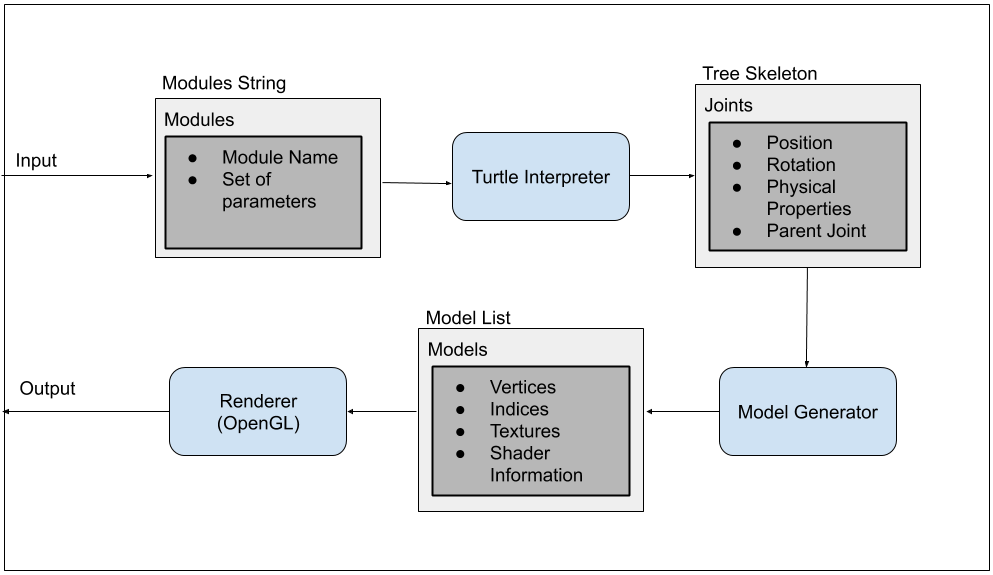
\includegraphics[scale=0.4]{Diagrams/L-systemInterpreter.png}
		\caption{Diagram of the stages of L-system interpretation and rendering} \label{l-system interpreter}
	}
\end{figure}
\FloatBarrier

\noindent
This chapter will cover each stage of the string interpreter implementation in detail, as well as well as talk about how the interpreter is able to simulate and animation the plants movements under forces such as gravity and wind in real time. 

\section{Turtle Graphics Interpreter}

The main purpose of the turtle graphics interpreter is to take the string of modules from the L-system rewriter, and interpret it as a list of turtle graphics instructions. As briefly covered in chapter \ref{l-system chapter}, each module name within the L-systems resultant string represents a particular meaning to the turtle graphics interpreter. The meaning of the module names are predefined in the string interpreter and are dependant on what the L-system is trying to represent. The L-system defined for this thesis is a parametric L-system, which allows each module to also provide a number of optional parameters. These may also carry a particular meaning for the interpreter. For instance the forward instruction or module name \say{F} can have three parameters. The value of the first parameter is the distance to move forward, this can also be seen as the length of the branch segment. The second and third parameter is the spring constant of the branch and the mass of the branch repectively. These give some information to the physics simulation in order to animate the plant. Below is a table describing the L-system module names as well as the parameter meanings for the turtle graphics interpreter.

\begin{table}[h!]
\centering
\begin{tabular}{ | c | l | l | l |}
\hline
	Instruction Name 	& Parameter 1 & Parameter 2 & Parameter 3 \\  
\hline
\hline
	F 							& Distance	& Spring Constant	& Branch Mass\\
\hline
	f 							& Distance	& Spring Constant	& Branch Mass\\
\hline
	+ 							& Angle of rotation &			&\\
\hline
	- 							& Angle	of rotation	&			&\\
\hline
	/ 							& Angle	of rotation	&			&\\
\hline
	$\backslash$ 				& Angle	of rotation	&			&\\
\hline
	$\land$ 					& Angle	of rotation	&			&\\
\hline
	\& 							& Angle	of rotation	&			&\\
\hline
	! 							& Branch width		&			&\\
\hline
\end{tabular}
\caption{Table of turtle instruction symbols and their meaning to the interpreter}
\label{instruction table 1}
\end{table}
\FloatBarrier

\noindent
Each modules instruction is carried out one by one to generate the plants skeletal structure, which is made up of joints. The joints hold information about the properties of each particular segement or object of the plant. The joints properties are the position, orientation, scale, parent joint as well as its physical characteristics. It is important to note that all of the scales and rotations must happen before the forward movement. As the rotations change the orientation of the brach and then the movement generates the joint itself. A joint is defined by the figure below:

\begin{figure}[htbp]
	{\centering
		\vspace{7px}
		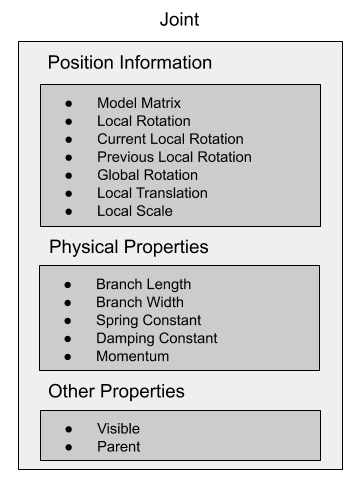
\includegraphics[scale=0.6]{Diagrams/JointDiagram.png}
		\caption{Diagram for the properties of a joint} \label{joint properties}
	}
\end{figure}
\FloatBarrier

\noindent
Figure \ref{joint properties} shows that there is in fact a large amount of information stored for the position and orientation of each joint. This is because the rotation of the joint is stored in both a local and global space. Local space refers to the rotation of the joint relative to its parent rotation, this is useful as it allows the manipulation of subsequent child joints, whilst leaving other joints local rotation unchanged. Global space, also known as world space, is the rotation of each joint relative to the world itself this is useful for understanding the current rotation of the joint relative to the world for instance calculating the torque or force calculations due to gravity. It is important to store both the current and previous rotations as they are used to calculate the rate of change for physics calculations.

The physical properties for each joint are the parts are what will affect model generation as well as physics simulations. These properties include the length, width, spring constant, damping constant as well as the current momentum of the branch. 

Take the following string of modules \say{F(1)[/(90)F(1)$\backslash$ (90)F(1)]-(90)F(1)+(90)F(1)}, the alphabet is made up of seven unique modules F, /, $\backslash$, [, ], + and -. According to the as discussed in previous chapters the \say{F} symbol represents a move forward, and \say{+}, \say{-}, \say{/}, \say{$\backslash$} symbolize different rotations, and the \say{[} and \say{]} represent save and load state respecively. The aforementioned symbols each have a single parameter except the load and save state. It is the turtle graphics interpreters job to understand what these parameters are and how to interpret them. In this case all of the \say{F} modules have the parameter value of 1, and all of the rotation modules have the parameter of 90. These are interpreted as the distance to move forward and the change in angle from the previous joint in degrees. This interpretation can be represented with the joint structure shown in figure \ref{skeleton diagram} below:

\begin{figure}[htbp]
	{\centering
		\vspace{7px}
		\setlength{\fboxrule}{1pt}
		\fbox{
			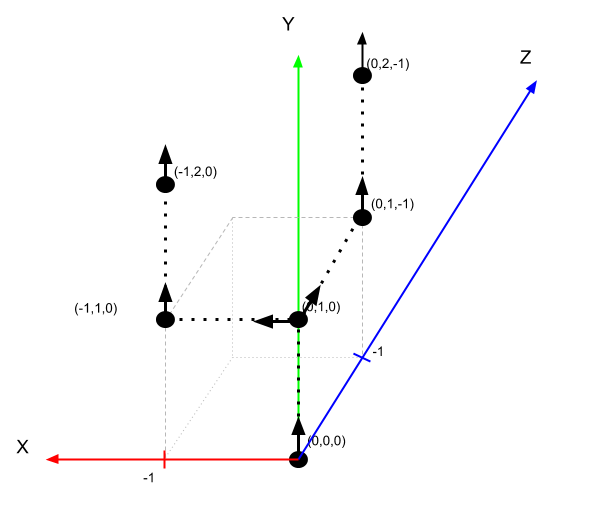
\includegraphics[scale=0.4]{Diagrams/SkeletonJoints.png}
		}
		\caption{Diagram of a simple plant skeleton with joint position and orientation.} \label{skeleton diagram}
	}
\end{figure}
\FloatBarrier


\section{3D Mathematics}

In any 3D application, mathematical models are used to represent the positions, rotations and scale of objects within a given scene. All objects within a 3D application are represented by a set of vertices or points, which can be represented with X, Y and Z coordinates. Three vertices can make up one triangle also called a face, multiple faces will then make up a whole 3D object. The use of mathematical methods in 3D graphics is to be able to manipulate all vertices of an object in a consistant way, thus rotating, translating or scaling the object within the scene. This section will provide sufficient background on some of most important concepts of 3D Mathematics, such as vectors, matrices and quaternions, which are widely used in the turtle graphics interpreter as well as the model generator.

\subsection{Vectors}

Vectors have many meanings in different contexts, in \acrshort{3d} computer graphics, often vectors are refering to the Euclidean vector. The Euclidean vector is a quantity in $n$-dimensional space that has both magnitude (the length from A to B) and direction (the direction to get from A to B). Vectors can be represented as a line segment pointing in a direction, with a certain length. A \acrshort{3d} vector can be written as a triple of scalar values eg: $(x, y, z)$

The most common operations on vectors are multiplication by a scalar, addition, subtraction, normalisation and the dot and cross product. The multiplication by a scalar value can be simply seen as scaling the magnitude of the vector itself, this can be done uniformly or non-uniformly as seen in the equation below:

\begin{equation}
a \otimes s = (a_x s_x, a_y s_y, a_z s_z)
\end{equation}

\noindent
Where $\otimes$ is the component-wise product of a vector $a$ and the scaling vector $s$. Similar to the scalar product of a vector the addition and subtraction of two vectors is the component-wise sum or difference. 

\begin{equation}
\begin{aligned}
a \oplus b = [(a_x + b_x), (a_y + b_y), (a_z + b_z)]\\
a \ominus b = [(a_x - b_x), (a_y - b_y), (a_z - b_z)]
\end{aligned}
\end{equation}

\begin{figure}[htbp]
	{\centering
		\setlength{\fboxrule}{1pt}
		\vspace{7px}
		\fbox{
			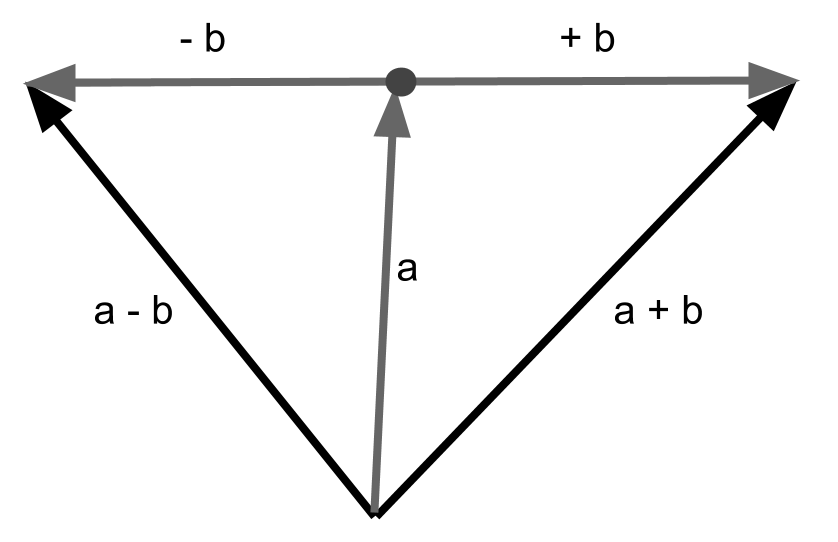
\includegraphics[scale=0.2]{Diagrams/vector_addition.png}
			\label{3DAxisFigure}
		}
		\caption{Table of common dot product tests between two vectors.}
	}
\end{figure}
\FloatBarrier

\noindent
A useful type of vector is known as a unit vector. This is a type of vector which has a magnitude of 1. Unit vectors are used extensively in computer graphics particularly with ragards to \gls{Shader}s. Take the vector v its magnitude $\alpha$ can be calculated by taking the square root of the product its components squared, as seen below 

\begin{equation}
	\alpha =~ \mid \textbf{v} \mid~ = \sqrt{\textbf{v}^2_x + \textbf{v}^2_y + \textbf{v}^2_z}
\end{equation}

The unit vector can then be calculated by taking the product of $v$ and the reciprocal of its magnitude shown in the following equation.

\begin{equation}
	\upsilon = \frac{\textbf{v}}{\alpha} = \frac{1}{\alpha} \textbf{v}
\end{equation}

There are many different ways to multiply vectors, however, in 3D graphics there two main multiplications. These being the dot and cross product. The dot product yields a scalar by adding the products of the vector product components. The cross product on the other hand is the product of two vectors which gives a vector which is perpendicular. The dot product can be calculated using the formula below: 

\begin{equation}
a \cdot b = a_x b_x + a_y b_y + a_z b_z = d
\end{equation}

\noindent
Some of the main uses for dot products within 3D graphics is to find whether two vectors are collinear, perpendicular, in the same direction or opposite directions. One possible use for this is to find the dot product of two branches directions in order to find out if they growing in the same direct or in opposite directions. In the table \ref{dot product test} below, there are each of the dot product test diagrams as well as the test equation where $ab = \mid a \mid \mid b \mid = a \cdot b$.

\begin{table}[h!]
\centering
\begin{tabular}{ | c | c | c |}
\hline
	Test 	& Equation & Example\\  
\hline
\hline
	Collinear 							& $(a \cdot b) = ab$ & 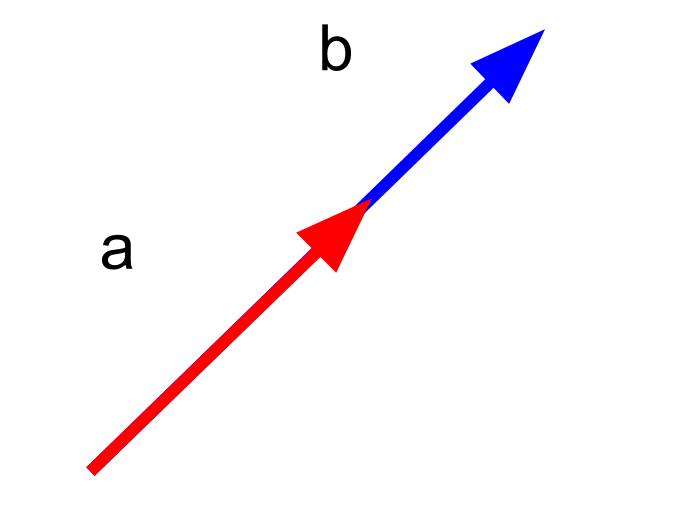
\includegraphics[scale=0.1]{Diagrams/vector1.png}\\
\hline
	Opposite Collinear 					& $(a \cdot b) = -ab$ &	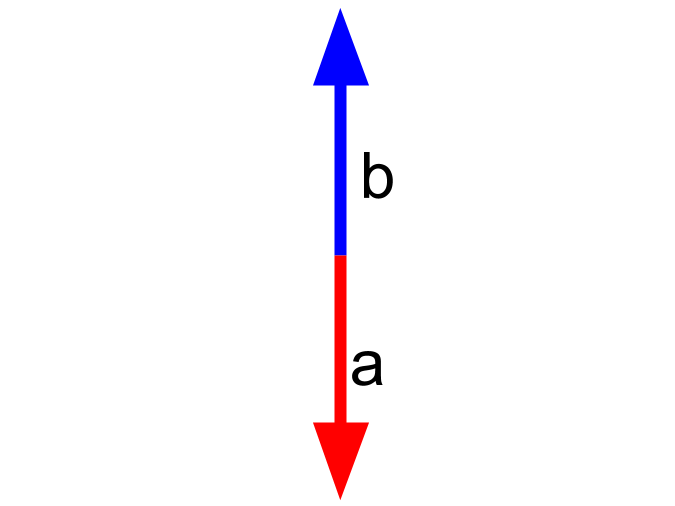
\includegraphics[scale=0.1]{Diagrams/vector2.png}\\
\hline
	Perpendicular 						& $(a \cdot b) = 0$	&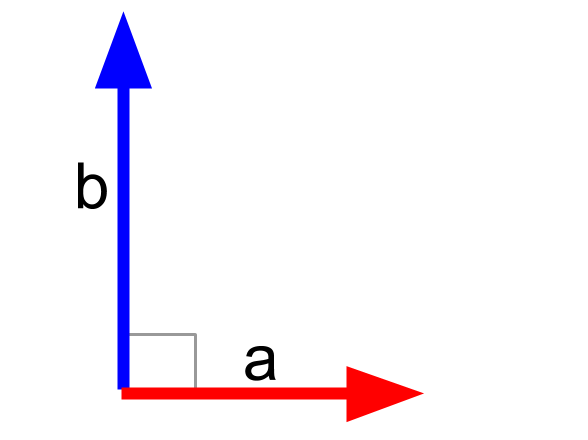
\includegraphics[scale=0.1]{Diagrams/vector3.png}\\
\hline
	Same Direction 						& $(a \cdot b) > 0$ &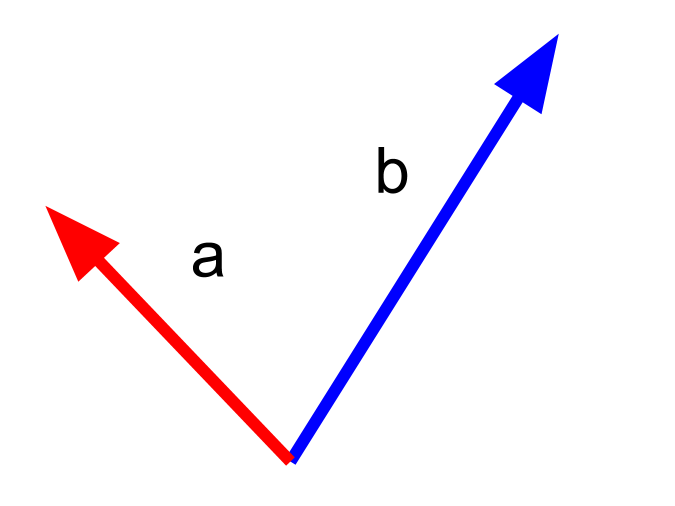
\includegraphics[scale=0.1]{Diagrams/vector4.png}\\
\hline
	Opposite Direction 					& $(a \cdot b) < 0$ &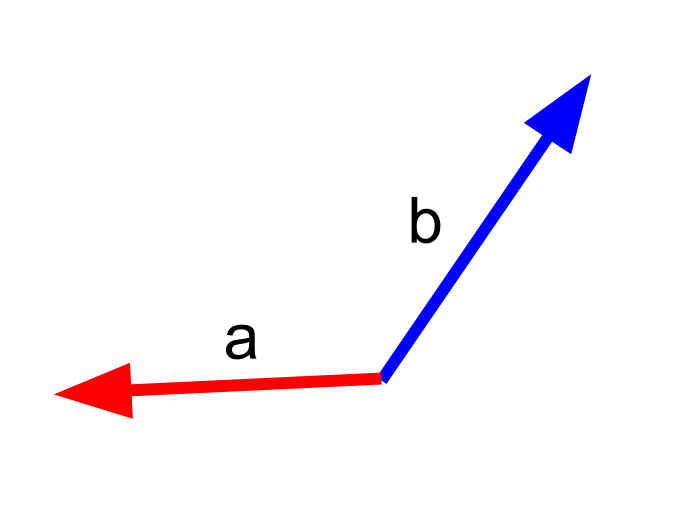
\includegraphics[scale=0.1]{Diagrams/vector5.png}\\
\hline

\end{tabular}
\caption{Table of turtle instruction symbols and their meaning to the interpreter}
\label{dot product test}
\end{table}
\FloatBarrier

\noindent
The cross product also known as the outer product takes two vectors and finds the perpendicular vector of the two vectors, this is only possible in 3D space and can be expressed in the following formula using the left-hand rule: 

\begin{equation}
a \times b = [(a_y b_z - a_z b_y), (a_z b_x - a_x b_z), (a_x b_y - a_y b_x)]
\end{equation}

\noindent
The result of a cross product can be seen in figure \ref{Cross product diagram} below. Where vectors $a$ and $b$ give the perpendicular vector $a \times b$. The cross product is very useful within physics calculations when it is necessary to find the rotational motion. 

\noindent
Some of the properties of the cross product are as follows:

\begin{itemize}
	\item is non-commutative, meaning order matters($a \times b \not= b \times a$).
	\item is anti-commutative ($a \times b = -(a \times b)$).
	\item is distributive with addition ($a \times (b + c) = (a \times b) + (a \times c)$).
\end{itemize}

\begin{figure}[htbp]
	{\centering
		\setlength{\fboxrule}{1pt}
		\vspace{7px}
		\fbox{
			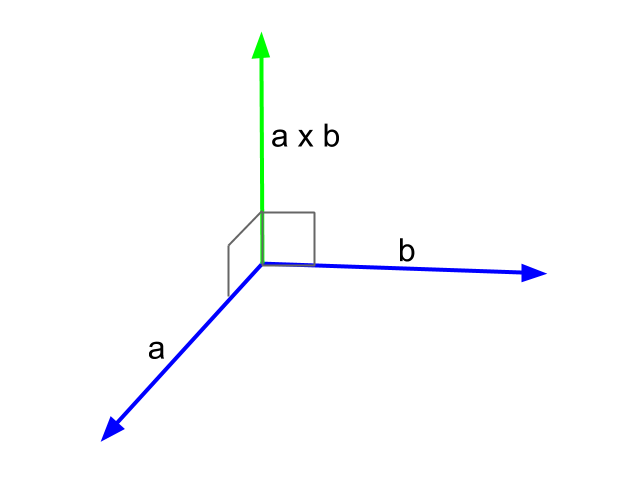
\includegraphics[scale=0.25]{Diagrams/cross_product.png}
			\label{Cross product diagram}
		}
		\caption{Diagram of the cross product of two vectors a and b.}
	}
\end{figure}
\FloatBarrier

\subsection{Matrices}

A model in 3D space will exist as a set of vertices which each have a position. Moving the model requires moving all of the the vertices of that model without distorting it in any way, this is called a model transform. There are four main types of transforms; translation, rotation, scale and shear. Matrices are a single matematical construct which is capable of carrying out all four of these transformations. This sections will only cover the first three as the shear transformation is likely not going to be useful for this thesis.    

A matrix is an 2D array of numbers, arranged into rows and columns, which can come in many different sizes. In 3D graphics, matrices used for transformations are the 3 $\times$ 3 and 4 $\times$ 4 matrix as seen below. A 3 $\times$ 3 matrix can be used for linear transorms such as scaling and rotation, furthermore, a linear transform which contains translation is known as an affine transform and can be represented by a 4 $\times$ 4 matrix known as an Atomic Transform Matrix. An atomic Transfom matrix is the concatination of four 4 $\times$ 4 matrices, one for translations, rotations, scale and shear transforms. Resulting in a 4 $\times$ 4 matrix as shown below. 

\begin{equation}
\textbf{M} = \begin{bmatrix}
M_{11} & M_{12} & M_{13} \\
M_{21} & M_{22} & M_{23} \\
M_{31} & M_{32} & M_{33}
\end{bmatrix}
\end{equation}

\begin{equation}
\textbf{M} = \begin{bmatrix}
M_{11} & M_{12} & M_{13} & M_{14}\\
M_{21} & M_{22} & M_{23} & M_{24}\\
M_{31} & M_{32} & M_{33} & M_{34}\\
M_{41} & M_{42} & M_{43} & M_{44}
\end{bmatrix}
\end{equation}

\noindent
The affine matrix can be shown in the expression below where $RS$ is a 3 $\times$ 3 matrix containing the rotation and scale where the $4^th$ elements are 0. The $T$ elements represent the translation with the 4th element being 1. 

\begin{equation}
\textbf{M} = \begin{bmatrix}
RS_{11} & RS_{12} & RS_{13} & 0\\
RS_{21} & RS_{22} & RS_{23} & 0\\
RS_{31} & RS_{32} & RS_{33} & 0\\
T_{1} & T_{2} & T_{3} & 1
\end{bmatrix}
\end{equation}

The product of two linear transform matrices will be another linear transform matrix that carries out both of those tranformations. This is true for the multiplication of two affine transform matrices as well, and is why matrix multiplication is so powerful in 3D graphics. Take the two matrices $A$ and $B$ which give the product $P$. In order to multiply $A$ and $B$ together, the dot product of the row and the column is calculated as seen below. It is also imporant to know that matrix multiplication is non-commutative $(AB \not= BA)$.

\begin{equation}
\textbf{AB} = \begin{bmatrix}
A_{11} & A_{12} & A_{13}\\
A_{21} & A_{22} & A_{23}\\
A_{31} & A_{32} & A_{33}
\end{bmatrix}
\times
\begin{bmatrix}
B_{11} & B_{12} & B_{13}\\
B_{21} & B_{22} & B_{23}\\
B_{31} & B_{32} & B_{33}
\end{bmatrix}
= \begin{bmatrix}
(A_{row1} \cdot B_{col1}) & (A_{row1} \cdot B_{col2}) & (A_{row1} \cdot B_{col3})\\
(A_{row2} \cdot B_{col1}) & (A_{row2} \cdot B_{col2}) & (A_{row2} \cdot B_{col3})\\
(A_{row3} \cdot B_{col1}) & (A_{row3} \cdot B_{col2}) & (A_{row3} \cdot B_{col3})
\end{bmatrix}
\end{equation}

To translate a vertex in 3D space without causing any distortion. The vertex can be added the the matrix below as follows. These translations can be carried out on all vertices in order to translate a whole object model. 

\begin{equation}
V + T = \begin{bmatrix}
V_{x} \\
V_{y} \\
V_{z}~ \\
1
\end{bmatrix}
+
\begin{bmatrix}
1 & 0 & 0 & 0\\
0 & 1 & 0 & 0\\
0 & 0 & 1 & 0\\
T_{x} & T_{y} & T_{z} & 1
\end{bmatrix}
= \begin{bmatrix}
(V_x + T_x)~ \\
(V_y + T_y)~ \\
(V_z + T_z)~ \\
1
\end{bmatrix}
\end{equation}

\noindent

In order to rotate a vertex in 3D space the vertex position and the rotation angle can be applied to the as a matrix depending on the axis about which it is rotating. These rotation matrices can be applied to the vertex itself in order to gain the new position of the vertex. 

\begin{equation}
R_x(\theta) = 
\begin{bmatrix}
(v_x)~ \\
(v_y)~ \\ 
(v_z)~ \\
1
\end{bmatrix}
\begin{bmatrix}
1 	& 0 					& 0 					& 0\\
0 	& \text{cos}(\theta) 	& \text{sin}(\theta) 	& 0\\
0 	& -\text{sin}(\theta) 	& \text{cos}(\theta) 	& 0\\
0 	& 0 					& 0 					& 1
\end{bmatrix}
\end{equation}

\begin{equation}
R_y(\theta) = 
\begin{bmatrix}
(v_x)~ \\
(v_y)~ \\
(v_z)~ \\
1
\end{bmatrix}
\begin{bmatrix}
\text{cos}(\theta) 	& 0 					& -\text{sin}(\theta) 	& 0\\
0 					& 1						& 0						& 0\\
\text{sin}(\theta) 	& 0 					& \text{cos}(\theta)	& 0\\
0 					& 0 					& 0 					& 1
\end{bmatrix}
\end{equation}

\begin{equation}
R_z(\theta) = 
\begin{bmatrix}
(v_x)~ \\
(v_y)~ \\
(v_z)~ \\
1
\end{bmatrix}
\begin{bmatrix}
\text{cos}(\theta) 	& \text{sin}(\theta) 	& 0						& 0\\
-\text{sin}(\theta) & \text{cos}(\theta) 	& 0
					& 0\\
0 					& 0 					& 1						& 0\\
0 					& 0 					& 0 					& 1
\end{bmatrix}
\end{equation}


\begin{equation}
ST = \begin{bmatrix}
S_{x} \\
S_{y} \\
S_{z} \\
1
\end{bmatrix}
\begin{bmatrix}
S_x & 0 & 0 & 0\\
0 & S_y & 0 & 0\\
0 & 0 & S_z & 0\\
0  & 0  & 0 & 1
\end{bmatrix}
= \begin{bmatrix}
(S_x R_x)~ \\
(S_y R_y)~ \\
(S_z R_z)~ \\
1
\end{bmatrix}
\end{equation}

\subsection{Quaternions}

In computer graphics there are a number of ways to represent 3D rotations. One method is to use matrices, as spoken about in the previous section. Matrices are often used to represent rotation, however, it has a number of limitations. Matrices are represented by nine floating point values and can be computationally expensive store and, process particularly when doing a vector to matrix multiplication. There are also situations where it is neccessary to smoothly transition from one rotation to another, or find a certain degree of rotation between two rotations. For example, when calculating the rotation of branch segments between time intervals in physics calculations. It is possible to make these calculations using matrices but it can become very complicated and even more computationally expensive. Quaterions are the miraculous answer to all of these difficulties.\\

Quaternions look similar to a 4D vector, as contains 4 axes $q = [qx, qy, qz, qw]$, these are represented with a real axis ($qw$) and three imaginary axis $qx, qy, qz$. A quaternion can be represented in complex form as follows: 

\begin{equation}
q = (iq_x + jq_y + kq_z + qw)
\end{equation}

For the purpose of this thesis it is not important to understand the derivation of quaterions in mathematics, however it is important to understand that any unit length quaternion which obays the rule in \ref{unit quat} below. 

\begin{equation} \label{unit quat}
	q_x^2 + q_y^2 + q_z^2 + q_w^2 = 1
\end{equation}

\noindent
Unit quaternions are used for rotations, it is possible to convert a quaternion to a unit quaternion  by taking the angle and the axis of a rotation and applying to the quaternion as follows: 

\begin{equation}
\begin{aligned}
& q = [qx, qy, qz]\\
& \text{where} \\
& q_x = a_x sin \frac{\theta}{2}\\
& q_y = a_y sin \frac{\theta}{2}\\
& q_z = a_z sin \frac{\theta}{2}\\
& q_w = cos \frac{\theta}{2}
\end{aligned}
\end{equation}

\noindent
The scalar part $q_w$ is the cosine of the half angle, and the vector part $q_x q_y q_z$ is the axis of that rotation, scaled by sine of the half angle of rotation. The unit quaternion can be used for rotations in a number of ways. The most useful of which is to rotate vectors, concatonate rotations together similar to how matrix transformations can be multiplied together as well as interpolate between two rotations. \\

The first operation for quaternions is that of addition. Simply the addition of two quaternions is just the component wise addition of the two quaternions, similar to that of matrices addition.

\begin{equation}
p + q = [(p_w + q_w), (p_x + q_x), (p_y + q_y), (p_z + q_z)]
\end{equation}

There are a number of types of quaternion multiplication, however, the one most commonly used for quaternion rotaton is called the grassmann product. This can be described in the following formula below. Where $p$ and $q$ are quaternions and the subscript $w$ indicates the scalar part and subscript $x, y, z$ indicate the vector components of each quaternion.

\begin{equation}
\begin{aligned}
R = r_w + r_x + r_y + r_z\\
\text{where}\\
r_w = p_w q_w - (p_x q_x + p_y q_y + p_z q_z)\\
r_x = p_w q_x + p_x q_w + p_y q_z - p_z q_y\\
r_y = p_w q_y + p_y q_w - p_x q_z + p_z q_x\\
r_z = p_w q_z + p_z q_w + p_x q_y - p_y q_x\\
\end{aligned}
\end{equation}

To rotate a vector by a unit quaternion the vector will need to be converted into its quaternion form. This requires taking the unit vector $v$ and using it as the vector part of the quaternion with a scalar part being equal to zero. This can be written as $Q_v = [v, 0] = [v_x, v_y, v_z, 0]$. In order to rotate the vector we can therefore take the grassmann product of the rotation quaternion $q$ and the vector form quaternion $v$ and the inverse of the rotation quaternion $q^-1$. \\

\begin{equation}
	V_q = qvq^{-1}
\end{equation}

\noindent
For unit quaternions the conjugate and the inverse are identical. The inverse of a unit quaternion can be calculated as follows. 

\begin{equation}
	q^{-1} = [-q_v, q_s]
\end{equation}


quaternion concatanation\\

rotational linear interpolation\\


\section{Model Generator}

Modeling the branches of a plant is one of the most important parts for the overall look and feel of that plant that is being generated. The L-system described in the previous sections is able to describe the details about the plants structure, for instance the position, width, length, weight and other important information. The job of the model generator is to take this information and intelligently generate the models vertices, normals, texture coordinates and other information that can then be provided to the OpenGL renderer and finally to the GPU to be rendered on the screen.

The simplest way to generate a model for a branching structure of a plant would be to take a number of cylinders, and to rotate and stack them according to each joints position in 3D space. The up side to this approach is that every branch within the plant shares the same object model, depending on the position, rotation and scale of the branch the relavent matrix transforms can be applied. In this way we are able to represent the overall branching structure of the plant. However, there is a problem which is pointed out by Baele and Warz\'{e}e "The branches junction causes a continuity problem: to simply stack up cylinders generates a gap" \cite{baele2005real}. This can be shown in the figure below:

\FloatBarrier

\begin{figure}[htbp]
	{\centering
		\vspace{7px}
		\setlength{\fboxrule}{1pt}
		\fbox{
			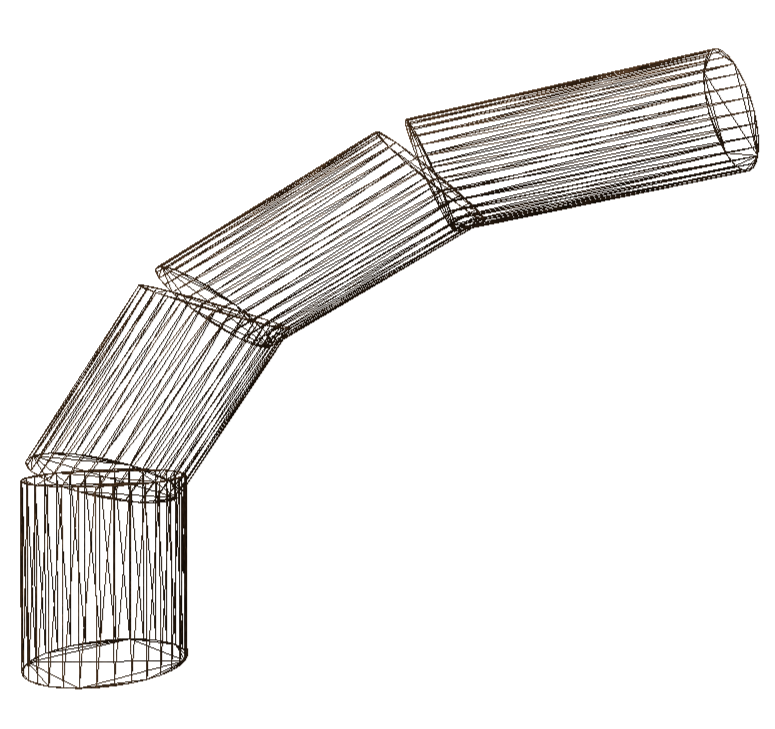
\includegraphics[scale=0.2]{Diagrams/stackedBranchesMesh.png}
		}
		\caption{Example of the continuity problem faced with stacked branching with a 25$^{\circ}$ bend per joint.}
	}
\end{figure}

\FloatBarrier

This simple method of stacking cylinders gives a reasonable looking tree structure and it is usually good enough when the angles of branches are not more than about 25$^{\circ}$ and the size of the branches do not change. However for a much more convincing tree structure we will want to do better than this. The logical next step would be to actively link the branch segments together.

\begin{figure}[htbp]
	{\centering
		\vspace{7px}
		\setlength{\fboxrule}{1pt}
		\fbox{
			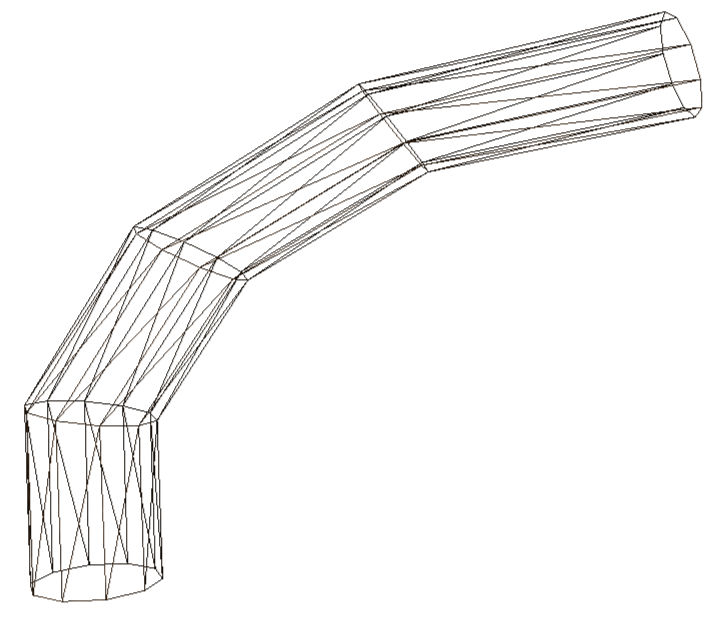
\includegraphics[scale=0.2]{Diagrams/linkedBranchesMesh.png}
		}
		\caption{Example of linked branching with a 25$^{\circ}$ bend per joint.}
	}
\end{figure}
\FloatBarrier

\section{Renderer}

The renderer is the final stage in the procedural generation pipeline. It takes all of the 3D models generated by the model generator, such as leaves, branches and flowers and renders them on the screen.  For this thesis, the \acrlong{opengl} (\acrshort{opengl}) application programming interface is use used to efficiently render the models on the screen using the \acrlong{gpu} (\acrshort{gpu}). 

The \acrshort{gpu} is a specially designed piece of harware for processing computer graphics and image processing, it has hundereds of individual compute cores which can be used in parallel. Due to the highly parallel nature of the \acrshort{gpu}, the \acrshort{opengl} framework helps to abstract the hardware and create an interface to interact with the \acrshort{gpu} in a simpler way. There are a number of other types of graphics \acrshort{api} such as Vulkan, Metal or DirectX. These \acrshort{api}s all provide a way of interacting with the hardware behind the scenes, However, they each have a different approach. Therefore, this section will not be be going into great detail about about the specifics of \acrshort{opengl} but rather the general concepts required for rendering the plant model on the screen.

\subsection{Models and Buffer Objects}

The model generator produces all of the information neccessary for the renderer to produce the result on the screen. In general the model data will consist of vertex data, texture co-ordinates and vertex normals. The vertex data is simply position of a point within a model, three vertices make up a face and the faces are what are ultimately rendered on the screen. The texture co-ordinates are the locations on a texture image which maps directly to the model vertices. Finally the vertex normals simply known as normals are the average normal vector. A normal vector being the vector that is purpendicular to the surface at a given point, and can be used for Phong shading or other types of lighting techniques.  

One of the most important parts of the rendering process is buffering the model data onto the \acrshort{gpu}. The \acrlong{vbo} (\acrshort{vbo}) is a data structure within the \acrshort{opengl} library which can be used to store this data on the \acrshort{gpu}. Generally, the data is stored as a single buffer or array with the first 3 values being a vertex position, the second two being a texture co-ordinate and the last three being a vertex normal. 

\begin{figure}[htbp]
	{\centering
		\vspace{7px}
		\setlength{\fboxrule}{1pt}
		\fbox{
			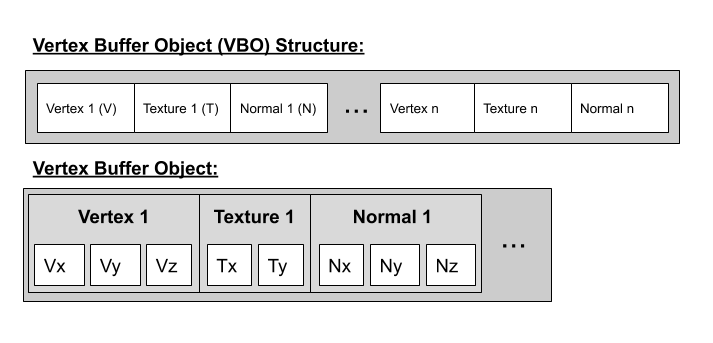
\includegraphics[scale=0.5]{Diagrams/VertexObjects.png}
		}
		\caption{Diagram showing the structure of a vertex buffer object.}
	}
\end{figure}
\FloatBarrier

 








